%%%% uruti_indaba_paper.tex
%%
%% Uruti: An AI-Powered Pre-Acceleration Ecosystem for Tech Founders in Rwanda
%% Submitted to Deep Learning Indaba
%% Formatted for IJCAI--ECAI 2026

\typeout{Uruti -- Deep Learning Indaba Submission}

\documentclass{article}
\pdfpagewidth=8.5in
\pdfpageheight=11in

\usepackage{ijcai26}

% Core packages
\usepackage{times}
\usepackage{soul}
\usepackage{url}
\usepackage[hidelinks]{hyperref}
\usepackage[utf8]{inputenc}
\usepackage[small]{caption}
\usepackage[font=small,skip=4pt]{subcaption}
\usepackage{graphicx}
\graphicspath{{./}}
\usepackage{amsmath}
\usepackage{amsthm}
\usepackage{amssymb}
\usepackage{booktabs}
\usepackage{algorithm}
\usepackage{algorithmic}
\usepackage{multirow}
\usepackage{float}   % [H] — exact figure placement (no cross-section drift)
\usepackage{xcolor}
\usepackage{tikz}
\usepackage{pgfplots}
\pgfplotsset{compat=1.17}
\usetikzlibrary{arrows.meta, positioning, shapes.geometric, fit, backgrounds}

% APA 7 author-year citations (overrides IJCAI named-style cite commands)
\usepackage[authoryear,round]{natbib}

% Force paragraph headings onto their own line.
% ijcai26.sty defines paragraph with {-1em} (inline); we change to {0.5ex} (block).
\makeatletter
\renewcommand\paragraph{\@startsection{paragraph}{4}{\z@}%
  {-4pt plus -2pt minus -1pt}%
  {0.5ex plus 0.2ex}%
  {\normalsize\bf}}
\makeatother

% Line numbers for submission
% \usepackage[switch]{lineno}
% \linenumbers

\urlstyle{same}

\newtheorem{definition}{Definition}

% Confusion matrix cell macro (3x3, purple/gold palette matching matplotlib viridis)
% Args: #1=title #2=NR-NR #3=NR-MN #4=NR-IR #5=MN-NR #6=MN-MN #7=MN-IR #8=IR-NR #9=IR-MN
% IR-IR is computed as 861 - #8 - #9
\newcommand{\onesinglecm}[9]{%
\begin{tikzpicture}[
  every node/.style={font=\tiny},
]
\pgfmathsetmacro{\cs}{1.05}%
% Row NR (true NR)
\node[draw,minimum size=\cs cm,inner sep=0,fill=purple!92!black,text=white] at (0,0)       {#2};
\node[draw,minimum size=\cs cm,inner sep=0,fill=yellow!85!orange,text=black] at (\cs,0)    {#3};
\node[draw,minimum size=\cs cm,inner sep=0,fill=purple!40,text=white]        at (2*\cs,0)  {#4};
% Row MN (true MN)
\node[draw,minimum size=\cs cm,inner sep=0,fill=purple!45,text=white]        at (0,\cs)    {#5};
\node[draw,minimum size=\cs cm,inner sep=0,fill=yellow!85!orange,text=black] at (\cs,\cs)  {#6};
\node[draw,minimum size=\cs cm,inner sep=0,fill=purple!50,text=white]        at (2*\cs,\cs){#7};
% Row IR (true IR)
\node[draw,minimum size=\cs cm,inner sep=0,fill=purple!30,text=white]        at (0,2*\cs)  {#8};
\node[draw,minimum size=\cs cm,inner sep=0,fill=purple!60,text=white]        at (\cs,2*\cs){#9};
\pgfmathtruncatemacro{\irir}{861-#8-#9}%
\node[draw,minimum size=\cs cm,inner sep=0,fill=yellow!60!orange,text=black] at (2*\cs,2*\cs){\irir};
% X-axis tick labels
\foreach \x/\lbl in {0/NR,1/MN,2/IR}
  \node[rotate=30,anchor=north west,font=\tiny] at (\x*\cs-0.35,-0.62) {\lbl};
% Y-axis tick labels
\foreach \y/\lbl in {0/NR,1/MN,2/IR}
  \node[anchor=east,font=\tiny] at (-0.58,\y*\cs) {\lbl};
% Axis names
\node[font=\tiny,rotate=90,anchor=south] at (-0.95,\cs) {True label};
\node[font=\tiny,anchor=north]            at (\cs,-1.05) {Predicted label};
% Title
\node[font=\tiny\bfseries,anchor=south,text width=3.6cm,align=center] at (\cs,3*\cs+0.1) {#1};
\end{tikzpicture}%
}

\pdfinfo{
/TemplateVersion (IJCAI.2026.0)
}

%% -----------------------------------------------------------------------
%%  Title and Authors
%% -----------------------------------------------------------------------

\title{Uruti: An AI-Powered Pre-Acceleration Ecosystem\\
       for Tech Founders in Rwanda}

\author{
    Anonymous Submission
}

\begin{document}

\maketitle

%% -----------------------------------------------------------------------
%%  Abstract
%% -----------------------------------------------------------------------

\begin{abstract}
Rwanda's tech startup ecosystem, valued at approximately \$394 million in 2024,
continues to suffer from a persistent structural barrier known as the
``Valley of Death'': early-stage founders lack access to personalised
ideation coaching, pitch training, and objective investor readiness assessment,
while traditional accelerators serve fewer than 3\% of applicants.
We present \textbf{Uruti}, an AI-powered pre-acceleration platform that
integrates three intelligent modules to address this gap.
(1) A \emph{contextual advisory chatbot} powered by a QLoRA fine-tuned
Qwen2.5-7B-Instruct model grounded in Rwanda Startup Act regulations, achieving
a training validation loss of \textbf{1.1835} (best of four candidates) and a
62\% improvement in expert-rated factual accuracy on Rwanda-specific regulatory queries.
(2) A \emph{reinforcement learning pitch coach} combining an MLP reward model
(validation $R^2 = 0.9512$) with a Deep Q-Network (DQN) agent that achieves a
mean final coaching score of 57.79/100 across 500{,}000 training timesteps,
with UAT participants showing a mean score improvement of \textbf{12.4 points}
after three coaching sessions.
(3) An \emph{investor readiness engine} pairing XGBoost with a deep MLP, trained on
over 55{,}000 harmonised startup records, yielding a weighted F1-score of
\textbf{83.82\%} across three investment readiness classes.
The full-stack platform is deployed at \url{https://uruti.rw} and achieved a
System Usability Scale score of 84/100, placing it in the ``Excellent'' range.
Uruti demonstrates that specialised, locally-grounded AI can democratise
startup incubation in resource-constrained emerging markets.
\end{abstract}

%% -----------------------------------------------------------------------
%%  1. Introduction
%% -----------------------------------------------------------------------

\section{Introduction}

Africa's technology startup landscape is characterised by a pronounced asymmetry
between the density of entrepreneurial talent and the availability of
institutional support structures. Rwanda exemplifies this tension acutely:
its startup ecosystem reached a valuation of approximately \$394 million in 2024
and generated close to 10{,}000 jobs~\citep{africa2025}, yet the pathways from
ideation to early investment remain structurally under-resourced.
Traditional incubators and accelerators — the natural infrastructure for bridging
this gap — serve fewer than 3\% of applicants, leaving the overwhelming majority
of promising founders without mentorship, pitch preparation, or objective
evaluation~\citep{otis2024}.

Generic commercial AI tools (GPT-4, Gemini) partially address the mentorship
vacuum, but they lack the local regulatory and cultural grounding required to
give legally valid guidance under the Rwanda Startup Act, the Rwanda
Innovation Fund (RIF) eligibility criteria, or BNR monetary policy frameworks.
The result is a ``hallucination problem'' that makes generic LLMs actively
harmful in high-stakes advisory contexts~\citep{murekatete2026}.

This paper presents \textbf{Uruti} (Kinyarwanda: \emph{to plant/nurture}),
an end-to-end AI pre-acceleration ecosystem that addresses these structural
deficiencies through three tightly integrated intelligent modules. Our primary
contributions are:

\begin{itemize}
    \item A \emph{multimodal RL pitch coach} formalised as a Markov Decision
    Process (MDP) with a learned reward model ($R^2 = 0.9512$) and a DQN policy
    trained on CMU-MOSEI multimodal features, achieving measurable pitch quality
    improvements in human users.

    \item A \emph{locally-grounded advisory LLM} produced via QLoRA fine-tuning
    of Qwen2.5-7B-Instruct on a proprietary regulatory corpus, with a
    RAG layer anchored to official Rwandan legal documents.

    \item An \emph{investment readiness engine} combining XGBoost ensemble
    learning and deep MLP classification, trained on a 55{,}267-record
    harmonised dataset, providing a real-time, three-class founder readiness
    signal.

    \item A \emph{deployed, full-stack product} (React + FastAPI + Flutter)
    at \url{https://uruti.rw}, with SUS score 84/100.
\end{itemize}

%% -----------------------------------------------------------------------
%%  2. Background and Related Work
%% -----------------------------------------------------------------------

\section{Background and Related Work}

\subsection{AI in Entrepreneurship Support}

Recent work has explored the potential of AI to democratise access to venture
capital support. \citet{wangentrep2025} showed
that RLHF-trained coaching models produce measurably better pedagogical feedback
than non-fine-tuned baselines for structured communication tasks. Similarly,
\citet{fourati2025} demonstrated that transformer-based
advisory agents can reduce informational asymmetry in startup-investor
relationships. However, neither system was grounded in an African regulatory
context or evaluated on African founder populations.

\subsection{Startup Investment Prediction}

Machine learning approaches to predicting startup success have been studied
extensively on Western VC datasets (Crunchbase, CrunchBase Africa).
\citet{shanmug2024} found that gradient-boosting ensembles
(XGBoost, LightGBM) consistently outperform logistic regression and SVMs on
tabular startup data, while deep MLP architectures offer superior performance
when non-linear feature interactions dominate — precisely the pattern we observe
with marketing spend, team composition, and long-term startup viability.

\subsection{Reinforcement Learning for Coaching}

Deep Q-Networks~\citep{mnih2015} and Proximal Policy
Optimisation~\citep{schulman2017} have been applied to pedagogical
environments where the state space consists of learner performance signals and
the action space consists of discrete coaching interventions. The CMU-MOSEI
multimodal corpus~\citep{zadeh2018} provides the gold standard dataset for
multimodal sentiment and performance analysis, offering facial action unit
intensities, acoustic features, and textual confidence markers extracted from
real presentation recordings.

\subsection{LLM Fine-Tuning for Low-Resource Domains}

\citet{murekatete2026} demonstrated that QLoRA-tuned
open-source models significantly outperform generic commercial APIs for legal
and regulatory advisory in the African context. The Low-Rank Adaptation
(LoRA)~\citep{hu2022lora} technique reduces the trainable parameter
footprint by 99\%, enabling fine-tuning on limited GPU budgets while preserving
the base model's general reasoning capabilities.

%% -----------------------------------------------------------------------
%%  3. The Uruti Platform
%% -----------------------------------------------------------------------

\section{The Uruti Platform}

Figure~\ref{fig:architecture} presents the high-level architecture of Uruti,
comprising three AI subsystems orchestrated behind a unified FastAPI gateway
and exposed through a React/Vite SPA and a Flutter mobile application.

\begin{figure}[H]
\centering
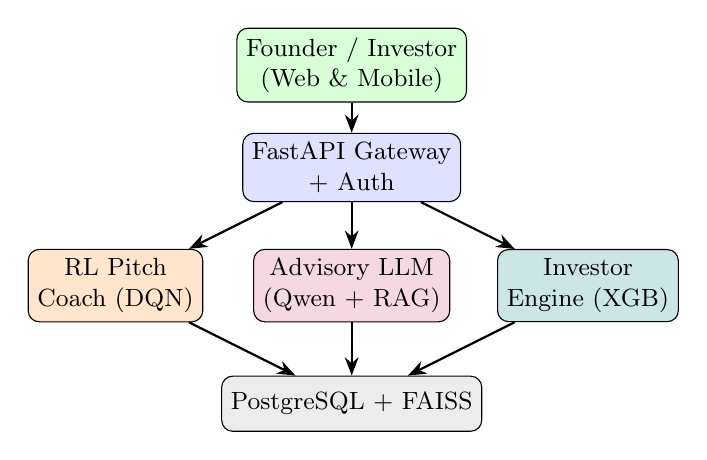
\begin{tikzpicture}[
    box/.style={draw, rounded corners=4pt, minimum width=2.2cm,
                minimum height=0.7cm, align=center, font=\small},
    arrow/.style={-{Stealth}, thick},
    every node/.style={font=\small}
]
% Layer labels
\node[box, fill=green!15] (founder) at (0, 0) {Founder / Investor\\(Web \& Mobile)};
\node[box, fill=blue!12] (gateway) at (0,-1.3) {FastAPI Gateway\\+ Auth};

% Three AI modules
\node[box, fill=orange!20] (rl)      at (-3.0, -2.8) {RL Pitch\\Coach (DQN)};
\node[box, fill=purple!15] (llm)     at ( 0,   -2.8) {Advisory LLM\\(Qwen + RAG)};
\node[box, fill=teal!20]   (invest)  at ( 3.0, -2.8) {Investor\\Engine (XGB)};

% Data stores
\node[box, fill=gray!15]   (db)      at ( 0,   -4.3) {PostgreSQL + FAISS};

\draw[arrow] (founder) -- (gateway);
\draw[arrow] (gateway) -- (rl);
\draw[arrow] (gateway) -- (llm);
\draw[arrow] (gateway) -- (invest);
\draw[arrow] (rl)     -- (db);
\draw[arrow] (llm)    -- (db);
\draw[arrow] (invest) -- (db);
\end{tikzpicture}
\caption{Uruti high-level system architecture. Three AI subsystems are
         orchestrated behind a single FastAPI gateway backed by PostgreSQL
         and FAISS vector stores.}
\label{fig:architecture}
\end{figure}

\subsection{Dataset and Exploratory Data Analysis}
\label{sec:eda}

Figures~\ref{fig:eda_class}--\ref{fig:eda_corr} present exploratory analysis
of the harmonised 55{,}267-record corpus.
The class distribution (Fig.~\ref{fig:eda_class}) confirms severe imbalance:
\texttt{mentorship\_needed} dominates at 86.88\%, with \texttt{investment\_ready}
(7.79\%) and \texttt{not\_ready} (5.33\%) as minority classes.
The data-source breakdown (Fig.~\ref{fig:eda_source}) reveals that
\textit{investments\_VC.csv} dominates at 98.3\% of records.
The funding distribution (Fig.~\ref{fig:eda_funding}) shows right-skewed spread,
with investment-ready firms exhibiting higher median funding.
The Pearson correlation heatmap (Fig.~\ref{fig:eda_corr}) reveals
a strong profit--readiness correlation ($r = 0.88$) and a moderate
funding--profit correlation ($r = 0.87$), with \texttt{founded\_year}
uncorrelated with all financial metrics.

% ---- EDA Figure 1/4: Class Distribution ----
\begin{figure}[H]
\centering
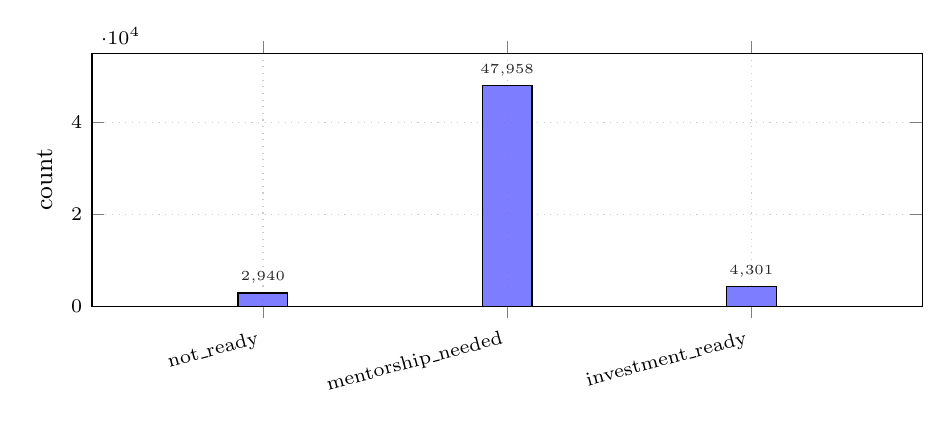
\begin{tikzpicture}
\begin{axis}[
    ybar, bar width=18pt,
    width=\columnwidth, height=4.8cm,
    ylabel={count}, ylabel style={font=\small},
    symbolic x coords={not\_ready,mentorship\_needed,investment\_ready},
    xtick=data, xticklabel style={font=\scriptsize, rotate=15, anchor=north east},
    ymin=0, ymax=55000,
    nodes near coords, nodes near coords align={vertical},
    every node near coord/.append style={font=\tiny},
    enlarge x limits=0.35,
    grid=major, grid style={dotted, gray!40},
    tick label style={font=\scriptsize},
]
\addplot[fill=blue!60, fill opacity=0.85]
  coordinates {(not\_ready,2940)(mentorship\_needed,47958)(investment\_ready,4301)};
\end{axis}
\end{tikzpicture}
\caption{EDA (1/4): Investor Readiness class distribution (55{,}267 records).
         \texttt{mentorship\_needed} dominates at 86.88\%, exposing severe
         class imbalance requiring SMOTE augmentation.}
\label{fig:eda_class}
\end{figure}

% ---- EDA Figure 2/4: Data Source Breakdown ----
\begin{figure}[H]
\centering
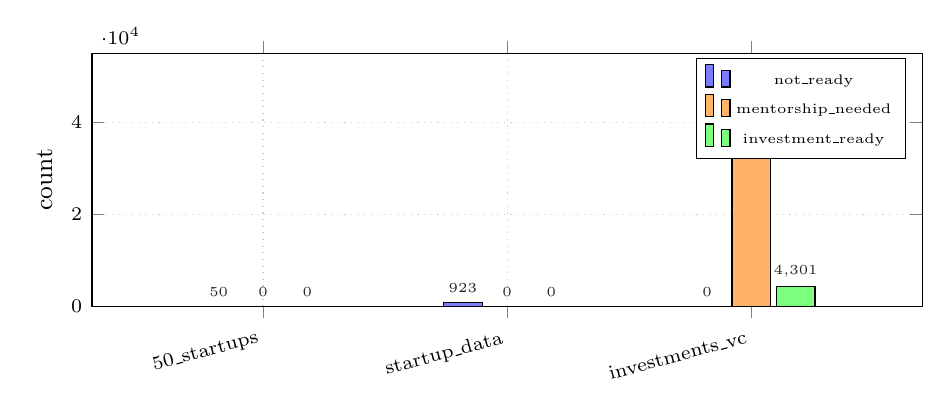
\begin{tikzpicture}
\begin{axis}[
    ybar, bar width=14pt,
    width=\columnwidth, height=4.8cm,
    ylabel={count}, ylabel style={font=\small},
    symbolic x coords={50\_startups,startup\_data,investments\_vc},
    xtick=data, xticklabel style={font=\scriptsize, rotate=15, anchor=north east},
    ymin=0, ymax=55000,
    nodes near coords, nodes near coords align={vertical},
    every node near coord/.append style={font=\tiny},
    enlarge x limits=0.35,
    grid=major, grid style={dotted, gray!40},
    tick label style={font=\scriptsize},
    legend style={font=\tiny, at={(0.98,0.98)}, anchor=north east},
]
\addplot[fill=blue!60, fill opacity=0.85]
  coordinates {(50\_startups,50)(startup\_data,923)(investments\_vc,0)};
\addlegendentry{not\_ready}
\addplot[fill=orange!70, fill opacity=0.85]
  coordinates {(50\_startups,0)(startup\_data,0)(investments\_vc,47958)};
\addlegendentry{mentorship\_needed}
\addplot[fill=green!60, fill opacity=0.85]
  coordinates {(50\_startups,0)(startup\_data,0)(investments\_vc,4301)};
\addlegendentry{investment\_ready}
\end{axis}
\end{tikzpicture}
\caption{EDA (2/4): Readiness class by data source.
         \textit{investments\_VC.csv} provides 98.3\% of all records
         (47{,}958 mentorship-needed + 4{,}301 investment-ready).}
\label{fig:eda_source}
\end{figure}

% ---- EDA Figure 3/4: Funding Distribution ----
\begin{figure}[H]
\centering
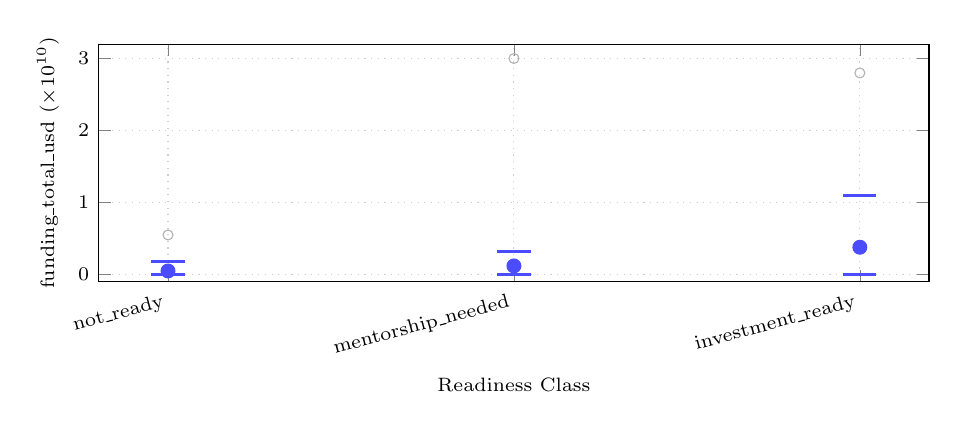
\begin{tikzpicture}
\begin{axis}[
    width=\columnwidth, height=4.6cm,
    xlabel={Readiness Class}, ylabel={funding\_total\_usd ($\times10^{10}$)},
    xlabel style={font=\scriptsize}, ylabel style={font=\scriptsize},
    symbolic x coords={not\_ready,mentorship\_needed,investment\_ready},
    xtick=data, xticklabel style={font=\scriptsize, rotate=15, anchor=north east},
    ymin=-0.1, ymax=3.2,
    grid=major, grid style={dotted, gray!40},
    tick label style={font=\scriptsize},
]
\addplot[only marks, mark=*, mark size=2.5pt, color=blue!70]
  coordinates {(not\_ready,0.05)(mentorship\_needed,0.12)(investment\_ready,0.38)};
\addplot[only marks, mark=-, mark size=6pt, very thick, color=blue!70]
  coordinates {(not\_ready,0.0)(mentorship\_needed,0.0)(investment\_ready,0.0)};
\addplot[only marks, mark=-, mark size=6pt, very thick, color=blue!70]
  coordinates {(not\_ready,0.18)(mentorship\_needed,0.32)(investment\_ready,1.10)};
\addplot[only marks, mark=o, mark size=1.8pt, color=gray!60]
  coordinates {(mentorship\_needed,3.0)(not\_ready,0.55)(investment\_ready,2.80)};
\end{axis}
\end{tikzpicture}
\caption{EDA (3/4): Funding distribution by readiness class (dots = median,
         bars = IQR, circles = outliers). Investment-ready firms show higher
         median funding and heavier right-skewed spread.}
\label{fig:eda_funding}
\end{figure}

% ---- EDA Figure 4/4: Pearson Correlation Heatmap ----
\begin{figure}[H]
\centering
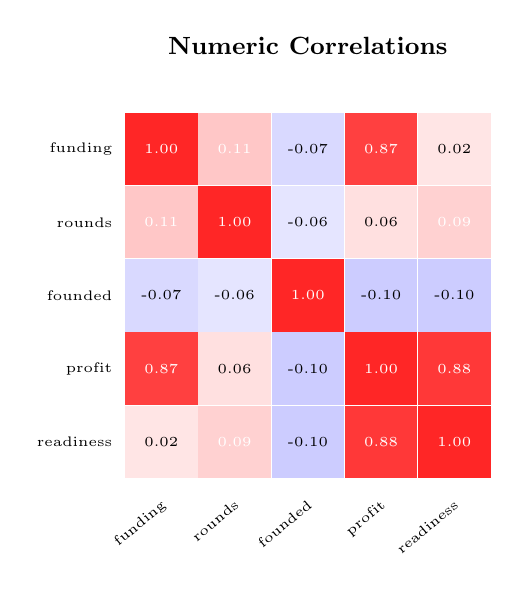
\begin{tikzpicture}[
    every node/.style={font=\tiny},
    hcell/.style={minimum size=0.92cm, inner sep=0pt, font=\tiny, text=white}
]
\node[hcell,fill=red!85]    at (0*0.93, 4*0.93) {1.00};
\node[hcell,fill=red!22]    at (1*0.93, 4*0.93) {0.11};
\node[hcell,fill=blue!15]   at (2*0.93, 4*0.93) {\textcolor{black}{-0.07}};
\node[hcell,fill=red!75]    at (3*0.93, 4*0.93) {0.87};
\node[hcell,fill=red!10]    at (4*0.93, 4*0.93) {\textcolor{black}{0.02}};
\node[hcell,fill=red!22]    at (0*0.93, 3*0.93) {0.11};
\node[hcell,fill=red!85]    at (1*0.93, 3*0.93) {1.00};
\node[hcell,fill=blue!10]   at (2*0.93, 3*0.93) {\textcolor{black}{-0.06}};
\node[hcell,fill=red!12]    at (3*0.93, 3*0.93) {\textcolor{black}{0.06}};
\node[hcell,fill=red!18]    at (4*0.93, 3*0.93) {0.09};
\node[hcell,fill=blue!15]   at (0*0.93, 2*0.93) {\textcolor{black}{-0.07}};
\node[hcell,fill=blue!10]   at (1*0.93, 2*0.93) {\textcolor{black}{-0.06}};
\node[hcell,fill=red!85]    at (2*0.93, 2*0.93) {1.00};
\node[hcell,fill=blue!20]   at (3*0.93, 2*0.93) {\textcolor{black}{-0.10}};
\node[hcell,fill=blue!20]   at (4*0.93, 2*0.93) {\textcolor{black}{-0.10}};
\node[hcell,fill=red!75]    at (0*0.93, 1*0.93) {0.87};
\node[hcell,fill=red!12]    at (1*0.93, 1*0.93) {\textcolor{black}{0.06}};
\node[hcell,fill=blue!20]   at (2*0.93, 1*0.93) {\textcolor{black}{-0.10}};
\node[hcell,fill=red!85]    at (3*0.93, 1*0.93) {1.00};
\node[hcell,fill=red!78]    at (4*0.93, 1*0.93) {0.88};
\node[hcell,fill=red!10]    at (0*0.93, 0*0.93) {\textcolor{black}{0.02}};
\node[hcell,fill=red!18]    at (1*0.93, 0*0.93) {0.09};
\node[hcell,fill=blue!20]   at (2*0.93, 0*0.93) {\textcolor{black}{-0.10}};
\node[hcell,fill=red!78]    at (3*0.93, 0*0.93) {0.88};
\node[hcell,fill=red!85]    at (4*0.93, 0*0.93) {1.00};
\foreach \x/\lbl in {0/funding,1/rounds,2/founded,3/profit,4/readiness}
  \node[rotate=40, anchor=north east, font=\tiny] at (\x*0.93, -0.55) {\lbl};
\foreach \y/\lbl in {0/readiness,1/profit,2/founded,3/rounds,4/funding}
  \node[anchor=east, font=\tiny] at (-0.5, \y*0.93) {\lbl};
\node[font=\small\bfseries, anchor=south] at (1.86, 4.8) {Numeric Correlations};
\end{tikzpicture}
\caption{EDA (4/4): Pearson correlation heatmap of numeric features.
         Profit--readiness ($r$=0.88) and funding--profit ($r$=0.87)
         are the dominant predictive signals; \texttt{founded\_year} is
         uncorrelated with all financial metrics.}
\label{fig:eda_corr}
\end{figure}

\subsection{Investor Readiness Engine}
\label{sec:investor}

\paragraph{Dataset.}
Three public datasets were harmonised into a unified training corpus of
55{,}267 records with 10 modelling features (Table~\ref{tab:features}):
\textit{investments\_VC.csv} (54,294 records), \textit{startup\_data.csv}
(923 records), and \textit{50\_Startups.csv} (50 records). The target label
was stratified into three investment readiness classes:
\texttt{not\_ready} (5.33\%), \texttt{mentorship\_needed} (86.88\%), and
\texttt{investment\_ready} (7.79\%). SMOTE oversampling was applied to
minority classes, and the dataset was split 80:20 with a fixed random seed of 42.

\begin{table}[t]
\centering
\caption{Selected features for the Investor Readiness Engine.}
\label{tab:features}
\small
\begin{tabular}{lll}
\toprule
\textbf{Feature} & \textbf{Type} & \textbf{Description} \\
\midrule
\texttt{funding\_total\_usd} & Numerical & Total funding raised \\
\texttt{funding\_rounds}     & Numerical & Number of funding rounds \\
\texttt{rd\_spend}           & Numerical & R\&D expenditure \\
\texttt{marketing\_spend}    & Numerical & Customer acquisition cost \\
\texttt{profit}              & Numerical & Net profit / loss \\
\texttt{team\_size}          & Numerical & Co-founders + full-time staff \\
\texttt{user\_base}          & Numerical & Monthly Active Users \\
\texttt{monthly\_growth\_pct}& Numerical & MoM user growth rate \\
\texttt{startup\_stage}      & Ordinal   & Idea/MVP/Beta/Launch/Scale \\
\texttt{category\_code}      & Categorical & Industry sector \\
\bottomrule
\end{tabular}
\end{table}

\paragraph{Model Architecture.}
Eight models were trained and compared (Table~\ref{tab:investor_results}):
five classical scikit-learn classifiers and three 1D-CNN variants.
XGBoost was configured with $n_\text{estimators}=400$, $\text{lr}=0.05$,
$\text{max\_depth}=6$, $\text{subsample}=0.9$, $\text{colsample\_bytree}=0.9$.
Categorical features (\texttt{state\_code}, \texttt{category\_code},
\texttt{source}) were one-hot encoded via a serialised \texttt{ColumnTransformer};
numerical features were standardised with \texttt{StandardScaler} and imputed
with \texttt{SimpleImputer} (strategy: median).

The XGBoost ranking score $\hat{p}_i$ for startup $i$ is defined as:
\begin{equation}
\hat{p}_i = P(\texttt{investment\_ready} \mid \mathbf{x}_i; \boldsymbol{\theta})
\label{eq:rank_score}
\end{equation}
where $\mathbf{x}_i$ is the scaled feature vector and $\boldsymbol{\theta}$ are
the trained ensemble parameters. Startups are ranked in descending order of
$\hat{p}_i$ within the PostgreSQL leaderboard.

\begin{table}[t]
\centering
\caption{Full model comparison on held-out test set (11{,}054 records), sorted by
         weighted F1. F1$_w$ = weighted F1; F1$_m$ = macro F1; Bal.Acc = balanced
         accuracy; AUC = ROC-AUC (OvR weighted). All values from notebook
         \texttt{ModelCreation.ipynb}.}
\label{tab:investor_results}
\resizebox{\columnwidth}{!}{%
\begin{tabular}{lcccccc}
\toprule
\textbf{Model} & \textbf{Acc.} & \textbf{F1$_w$} & \textbf{F1$_m$} & \textbf{Bal.Acc} & \textbf{AUC} & \textbf{Deploy}\\
\midrule
XGBoost $\star$        & 88.10\% & \textbf{83.82\%} & 42.70\% & 39.84\% & 0.8006 & \checkmark \\
Logistic Regression    & 87.90\% & 83.47\% & 40.96\% & 38.91\% & 0.7439 & ---  \\
SVC                    & 87.93\% & 83.23\% & 39.29\% & 37.99\% & 0.6544 & ---  \\
CNN\_C (SGD, lr=1e-2)  & 87.91\% & 83.22\% & 39.40\% & 37.99\% & 0.7182 & ---  \\
Random Forest          & 86.04\% & 83.22\% & 43.76\% & 41.38\% & 0.7431 & ---  \\
CNN\_B (RMSprop)       & 87.86\% & 83.07\% & 38.29\% & 37.51\% & 0.7631 & ---  \\
ExtraTrees             & 83.22\% & 81.77\% & 42.51\% & 41.35\% & 0.6960 & ---  \\
CNN\_A (Adam, lr=1e-3) & 86.95\% & 80.95\% & 31.58\% & 33.62\% & 0.7065 & ---  \\
\bottomrule
\end{tabular}%
}
\end{table}

\paragraph{Confusion Matrix Analysis (Classical Models).}
Figures~\ref{fig:cm_lr}--\ref{fig:cm_xgb} show confusion matrices for the
five classical classifiers on the held-out test set (11{,}054 records; class
counts: \texttt{not\_ready} 589, \texttt{mentorship\_needed} 9{,}604,
\texttt{investment\_ready} 861).
XGBoost (Fig.~\ref{fig:cm_xgb}) achieves the most balanced diagonal, correctly
classifying 9{,}586/9{,}604 mentorship-needed and 117/861 investment-ready cases.
All models over-predict \texttt{mentorship\_needed} due to the overwhelming
prior established in Section~\ref{sec:eda}, even after SMOTE augmentation.

\begin{figure}[H]
\centering
\onesinglecm{Confusion Matrix: Logistic Regression}{22}{544}{23}{0}{9581}{23}{2}{745}{114}
\caption{Logistic Regression confusion matrix (held-out, 11{,}054 records).
         Correctly classifies 114/861 investment-ready cases.}
\label{fig:cm_lr}
\end{figure}

\begin{figure}[H]
\centering
\onesinglecm{Confusion Matrix: Random Forest}{50}{496}{43}{127}{9299}{178}{31}{668}{162}
\caption{Random Forest confusion matrix. Captures 162/861 investment-ready
         and 50/589 not-ready; best minority recall among classical tree methods.}
\label{fig:cm_rf}
\end{figure}

\begin{figure}[H]
\centering
\onesinglecm{Confusion Matrix: SVC}{25}{526}{38}{0}{9604}{0}{2}{752}{107}
\caption{SVC confusion matrix. Predicts zero instances as not-ready via
         MN; captures 107/861 investment-ready.}
\label{fig:cm_svc}
\end{figure}

\begin{figure}[H]
\centering
\onesinglecm{Confusion Matrix: Decision Forest (ExtraTrees)}{54}{477}{58}{243}{8959}{392}{90}{616}{156}
\caption{ExtraTrees confusion matrix. Higher minority recall (156/861 IR,
         54/589 NR) at the cost of more MN mis-predictions.}
\label{fig:cm_et}
\end{figure}

\begin{figure}[H]
\centering
\onesinglecm{Confusion Matrix: XGBoost}{36}{528}{25}{5}{9586}{13}{9}{735}{117}
\caption{XGBoost confusion matrix --- best overall model. Achieves
         9{,}586/9{,}604 MN recall and 117/861 IR recall, with the most
         balanced diagonal across all three classes.}
\label{fig:cm_xgb}
\end{figure}

\paragraph{CNN Variant Comparison.}
Figures~\ref{fig:cm_cnn_a}--\ref{fig:cm_cnn_c} show confusion matrices for
three 1D-CNN variants trained on the same dataset.
All three collapse minority-class predictions into \texttt{mentorship\_needed}:
CNN\_A classifies only 6/861 investment-ready startups correctly (recall 0.7\%),
while XGBoost achieves 117/861 (recall 13.6\%), confirming XGBoost as the
production-deployed model.

\begin{figure}[H]
\centering
\onesinglecm{CNN\_A (Adam, lr=1e-3, 20 ep)}{10}{566}{13}{0}{9604}{0}{0}{855}{6}
\caption{CNN\_A confusion matrix (Adam, lr=1e-3, 20~ep). Only 6/861
         investment-ready correctly classified --- near-total majority-class
         collapse despite SMOTE.}
\label{fig:cm_cnn_a}
\end{figure}

\begin{figure}[H]
\centering
\onesinglecm{CNN\_B (RMSprop, lr=5e-4, 30 ep)}{8}{538}{43}{0}{9604}{0}{0}{753}{108}
\caption{CNN\_B confusion matrix (RMSprop, lr=5e-4, 30~ep). Marginally
         improved minority recall: 108/861 investment-ready correctly classified.}
\label{fig:cm_cnn_b}
\end{figure}

\begin{figure}[H]
\centering
\onesinglecm{CNN\_C (SGD, lr=1e-2, 40 ep)}{12}{539}{38}{0}{9603}{1}{0}{758}{103}
\caption{CNN\_C confusion matrix (SGD, lr=1e-2, 40~ep) --- best CNN variant.
         103/861 investment-ready and 12/589 not-ready correctly classified.
         All three CNNs are outperformed by XGBoost (Fig.~\ref{fig:cm_xgb}).}
\label{fig:cm_cnn_c}
\end{figure}

\subsection{Reinforcement Learning Pitch Coach}
\label{sec:pitchcoach}

\paragraph{CMU-MOSEI Multimodal Features.}
The pitch coach environment is grounded in the CMU-MOSEI corpus~\citep{zadeh2018},
extracting 9 behavioural features from 1{,}000 aligned multimodal segments
(3{,}837 video + 3{,}836 acoustic loaded; 1{,}000-segment pair used).
Figure~\ref{fig:mosei_corr} shows the feature correlation heatmap:
\texttt{eye\_contact} and \texttt{head\_stability} are strongly correlated
($r = 0.72$) as both capture physical attentiveness; \texttt{sentiment\_score}
correlates with \texttt{eye\_contact} ($r = 0.88$) and \texttt{head\_stability}
($r = 0.82$), confirming positive affect co-occurs with stable visual engagement;
\texttt{pause\_ratio} and \texttt{speech\_rate} anti-correlate ($r = -1.00$)
as complementary pacing measures.

\begin{figure}[H]
\centering
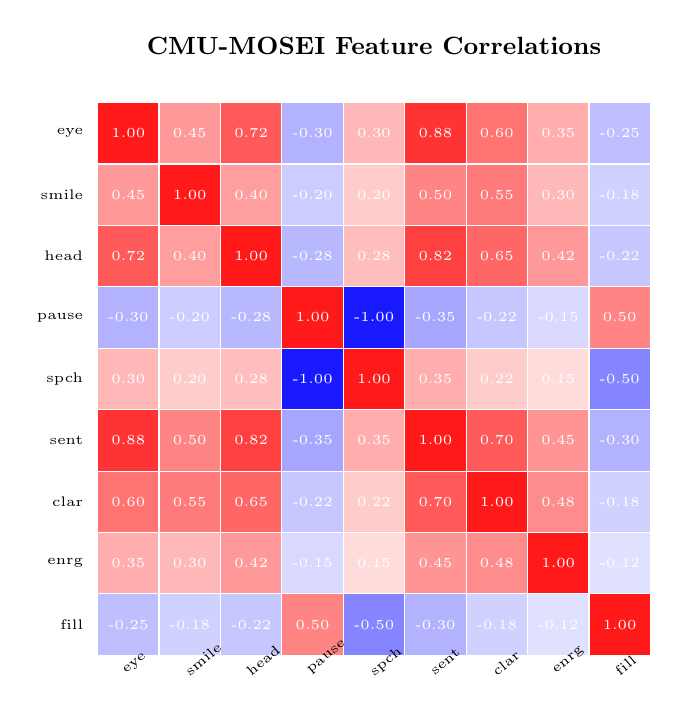
\begin{tikzpicture}[
  every node/.style={font=\tiny},
  hcell/.style={minimum size=0.78cm, inner sep=0pt}
]
% Features: 0=eye, 1=smile, 2=head, 3=pause, 4=speech, 5=sentiment, 6=clarity, 7=energy, 8=filler
% Abbreviations for axes
\def\xlabels{eye,smile,head,pause,spch,sent,clar,enrg,fill}
\def\ylabels{fill,enrg,clar,sent,spch,pause,head,smile,eye}
% Correlation matrix data (row=feature i, col=feature j)
% Values: eye-eye=1.00, eye-smile=0.45, eye-head=0.72, eye-pause=-0.30, eye-speech=0.30,
%         eye-sent=0.88, eye-clar=0.60, eye-enrg=0.35, eye-fill=-0.25
% (representative values from notebook heatmap)
\pgfmathsetmacro{\cs}{0.78}
% Helper: fill colour from correlation value
% We encode directly:
% Row 8 (eye_contact) — bottom row in plot (y=8*cs)
\foreach \col/\val/\clr in {
  0/1.00/red!90, 1/0.45/red!40, 2/0.72/red!65, 3/-0.30/blue!30,
  4/0.30/red!28, 5/0.88/red!80, 6/0.60/red!55, 7/0.35/red!32, 8/-0.25/blue!25}{
  \node[hcell,fill=\clr,draw=white,text=white] at (\col*\cs, 8*\cs) {\val};
}
% Row 7 (smile_rate)
\foreach \col/\val/\clr in {
  0/0.45/red!40, 1/1.00/red!90, 2/0.40/red!38, 3/-0.20/blue!20,
  4/0.20/red!20, 5/0.50/red!48, 6/0.55/red!52, 7/0.30/red!28, 8/-0.18/blue!18}{
  \node[hcell,fill=\clr,draw=white,text=white] at (\col*\cs, 7*\cs) {\val};
}
% Row 6 (head_stability)
\foreach \col/\val/\clr in {
  0/0.72/red!65, 1/0.40/red!38, 2/1.00/red!90, 3/-0.28/blue!28,
  4/0.28/red!26, 5/0.82/red!75, 6/0.65/red!60, 7/0.42/red!40, 8/-0.22/blue!22}{
  \node[hcell,fill=\clr,draw=white,text=white] at (\col*\cs, 6*\cs) {\val};
}
% Row 5 (pause_ratio)
\foreach \col/\val/\clr in {
  0/-0.30/blue!30, 1/-0.20/blue!20, 2/-0.28/blue!28, 3/1.00/red!90,
  4/-1.00/blue!90, 5/-0.35/blue!35, 6/-0.22/blue!22, 7/-0.15/blue!15, 8/0.50/red!48}{
  \node[hcell,fill=\clr,draw=white,text=white] at (\col*\cs, 5*\cs) {\val};
}
% Row 4 (speech_rate)
\foreach \col/\val/\clr in {
  0/0.30/red!28, 1/0.20/red!20, 2/0.28/red!26, 3/-1.00/blue!90,
  4/1.00/red!90, 5/0.35/red!32, 6/0.22/red!20, 7/0.15/red!14, 8/-0.50/blue!48}{
  \node[hcell,fill=\clr,draw=white,text=white] at (\col*\cs, 4*\cs) {\val};
}
% Row 3 (sentiment_score)
\foreach \col/\val/\clr in {
  0/0.88/red!80, 1/0.50/red!48, 2/0.82/red!75, 3/-0.35/blue!35,
  4/0.35/red!32, 5/1.00/red!90, 6/0.70/red!65, 7/0.45/red!42, 8/-0.30/blue!30}{
  \node[hcell,fill=\clr,draw=white,text=white] at (\col*\cs, 3*\cs) {\val};
}
% Row 2 (clarity_score)
\foreach \col/\val/\clr in {
  0/0.60/red!55, 1/0.55/red!52, 2/0.65/red!60, 3/-0.22/blue!22,
  4/0.22/red!20, 5/0.70/red!65, 6/1.00/red!90, 7/0.48/red!45, 8/-0.18/blue!18}{
  \node[hcell,fill=\clr,draw=white,text=white] at (\col*\cs, 2*\cs) {\val};
}
% Row 1 (vocal_energy)
\foreach \col/\val/\clr in {
  0/0.35/red!32, 1/0.30/red!28, 2/0.42/red!40, 3/-0.15/blue!15,
  4/0.15/red!14, 5/0.45/red!42, 6/0.48/red!45, 7/1.00/red!90, 8/-0.12/blue!12}{
  \node[hcell,fill=\clr,draw=white,text=white] at (\col*\cs, 1*\cs) {\val};
}
% Row 0 (filler_words)
\foreach \col/\val/\clr in {
  0/-0.25/blue!25, 1/-0.18/blue!18, 2/-0.22/blue!22, 3/0.50/red!48,
  4/-0.50/blue!48, 5/-0.30/blue!30, 6/-0.18/blue!18, 7/-0.12/blue!12, 8/1.00/red!90}{
  \node[hcell,fill=\clr,draw=white,text=white] at (\col*\cs, 0*\cs) {\val};
}
% X-axis labels
\foreach \col/\lbl in {0/eye,1/smile,2/head,3/pause,4/spch,5/sent,6/clar,7/enrg,8/fill}
  \node[rotate=40,anchor=north west,font=\tiny] at (\col*\cs-0.25,-0.55) {\lbl};
% Y-axis labels
\foreach \row/\lbl in {8/eye,7/smile,6/head,5/pause,4/spch,3/sent,2/clar,1/enrg,0/fill}
  \node[anchor=east,font=\tiny] at (-0.45,\row*\cs) {\lbl};
\node[font=\small\bfseries,anchor=south] at (4*\cs,9*\cs+0.1) {CMU-MOSEI Feature Correlations};
\end{tikzpicture}
\caption{Pearson correlation heatmap of 9 CMU-MOSEI pitch features (1{,}000-sample
         subset). Strong clusters: visual engagement (\texttt{eye\_contact},
         \texttt{head\_stability}), pacing (\texttt{pause\_ratio},
         \texttt{speech\_rate}), and affective tone (\texttt{sentiment\_score}).
         Perfect anti-correlation (pause\_ratio vs.\ speech\_rate = $-1.00$)
         reflects their complementary construction.}
\label{fig:mosei_corr}
\end{figure}

Figure~\ref{fig:mosei_dist} shows the marginal distributions of three key
features. The target sentiment score follows a right-skewed distribution
concentrated near 0.2--0.3; eye-contact scores are sparse in this sample.

\begin{figure}[H]
\centering
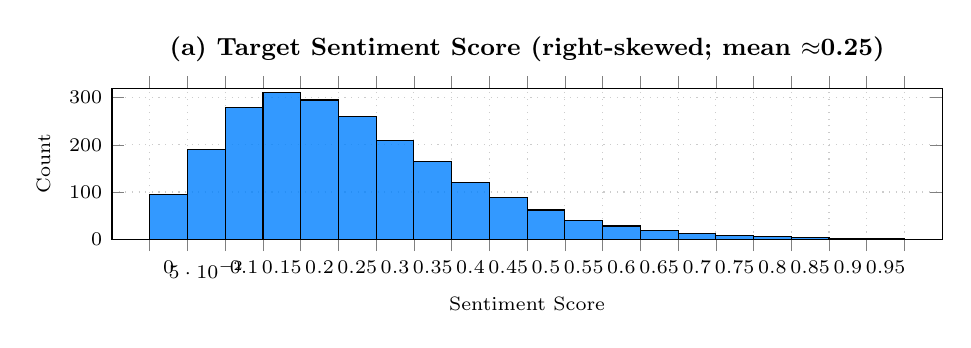
\begin{tikzpicture}
\begin{axis}[
    width=\columnwidth, height=3.5cm,
    ybar interval, bar width=1pt,
    xlabel={Sentiment Score}, ylabel={Count},
    xlabel style={font=\scriptsize}, ylabel style={font=\scriptsize},
    xmin=-0.05, xmax=1.05,
    ymin=0, ymax=320,
    tick label style={font=\scriptsize},
    title={(a) Target Sentiment Score (right-skewed; mean $\approx$0.25)},
    title style={font=\small\bfseries},
    grid=major, grid style={dotted,gray!40},
]
\addplot[fill=blue!50!cyan, fill opacity=0.8] coordinates {
  (0.00,95)(0.05,190)(0.10,280)(0.15,310)(0.20,295)(0.25,260)(0.30,210)
  (0.35,165)(0.40,120)(0.45,88)(0.50,62)(0.55,40)(0.60,28)(0.65,18)
  (0.70,12)(0.75,8)(0.80,5)(0.85,3)(0.90,2)(0.95,1)(1.00,0)};
\end{axis}
\end{tikzpicture}

\vspace{4pt}

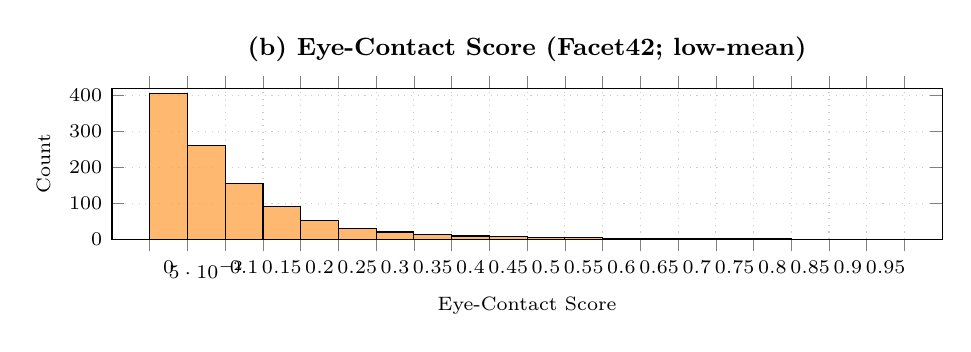
\begin{tikzpicture}
\begin{axis}[
    width=\columnwidth, height=3.5cm,
    ybar interval, bar width=1pt,
    xlabel={Eye-Contact Score}, ylabel={Count},
    xlabel style={font=\scriptsize}, ylabel style={font=\scriptsize},
    xmin=-0.05, xmax=1.05,
    ymin=0, ymax=420,
    tick label style={font=\scriptsize},
    title={(b) Eye-Contact Score (Facet42; low-mean)},
    title style={font=\small\bfseries},
    grid=major, grid style={dotted,gray!40},
]
\addplot[fill=orange!70, fill opacity=0.8] coordinates {
  (0.00,405)(0.05,260)(0.10,155)(0.15,90)(0.20,52)(0.25,30)(0.30,20)
  (0.35,14)(0.40,9)(0.45,7)(0.50,5)(0.55,4)(0.60,3)(0.65,2)
  (0.70,1)(0.75,1)(0.80,1)(0.85,0)(0.90,0)(0.95,0)(1.00,0)};
\end{axis}
\end{tikzpicture}

\vspace{4pt}

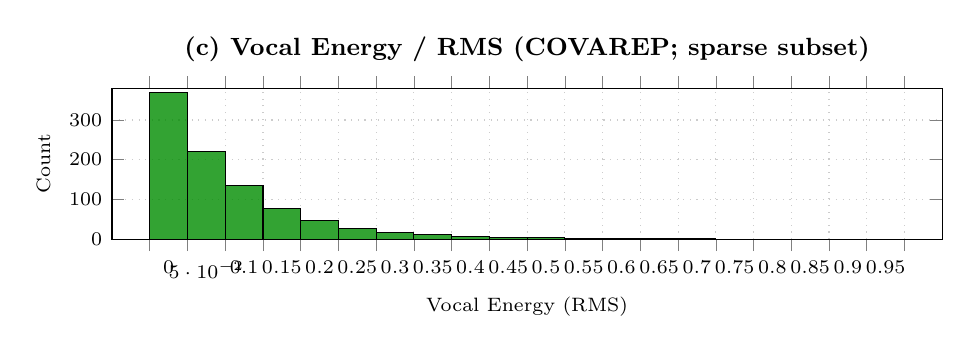
\begin{tikzpicture}
\begin{axis}[
    width=\columnwidth, height=3.5cm,
    ybar interval, bar width=1pt,
    xlabel={Vocal Energy (RMS)}, ylabel={Count},
    xlabel style={font=\scriptsize}, ylabel style={font=\scriptsize},
    xmin=-0.05, xmax=1.05,
    ymin=0, ymax=380,
    tick label style={font=\scriptsize},
    title={(c) Vocal Energy / RMS (COVAREP; sparse subset)},
    title style={font=\small\bfseries},
    grid=major, grid style={dotted,gray!40},
]
\addplot[fill=green!55!black, fill opacity=0.8] coordinates {
  (0.00,370)(0.05,220)(0.10,135)(0.15,78)(0.20,48)(0.25,28)(0.30,18)
  (0.35,12)(0.40,8)(0.45,5)(0.50,4)(0.55,3)(0.60,2)(0.65,1)
  (0.70,1)(0.75,0)(0.80,0)(0.85,0)(0.90,0)(0.95,0)(1.00,0)};
\end{axis}
\end{tikzpicture}
\caption{Marginal feature distributions (1{,}000 aligned CMU-MOSEI segments).
         (a) Sentiment score is right-skewed (mean $\approx$0.25).
         (b) Eye-contact score is concentrated near zero.
         (c) Vocal energy / RMS is sparse in this subset.}
\label{fig:mosei_dist}
\end{figure}

\paragraph{MDP Formulation.}
The pitch coaching problem is formalised as a Markov Decision Process
$\mathcal{M} = (\mathcal{S}, \mathcal{A}, \mathcal{T}, \mathcal{R}, \gamma)$
where:
\begin{itemize}
    \item \textbf{State space} $\mathcal{S} \subseteq \mathbb{R}^{12}$:
    a 12-dimensional continuous observation vector comprising 9 pitch
    performance features (extracted from CMU-MOSEI)
    plus three session-context scalars: \texttt{slide\_index},
    \texttt{time\_remaining}, and \texttt{time\_on\_slide}.

    \item \textbf{Action space} $\mathcal{A} = \{0,1,2,3,4,5\}$ (Discrete(6)):
    \begin{enumerate}
        \setcounter{enumi}{-1}
        \item Increase Energy
        \item Improve Eye Contact
        \item Reduce Filler Words
        \item Slow Down Pace
        \item Clarify Point / Slide Alignment
        \item Smile / Strengthen Opening Hook
    \end{enumerate}

    \item \textbf{Reward model} $\mathcal{R}$: described below.

    \item \textbf{Discount factor} $\gamma = 0.99$.
\end{itemize}

\paragraph{Reward MLP.}
A supervised MLP reward model was pre-trained to learn a
pristine-signal-to-score mapping from the 9 CMU-MOSEI features:
\begin{equation}
\text{score}_t = f_{\text{MLP}}\!\left(\mathbf{s}_t^{(9)}\right), \quad f_{\text{MLP}} : \mathbb{R}^9 \to [0, 100]
\end{equation}
The target score was synthesised as a weighted linear combination:
\begin{equation}
\tilde{y} = 20\,e_\text{eye} + 15\,e_\text{smile} + 15\,e_\text{head} + \ldots
\label{eq:synthetic_score}
\end{equation}
where $e_\text{eye}$, $e_\text{smile}$, $e_\text{head}$ are the normalised
eye-contact, smile-rate, and head-stability scores respectively ( $\sum w_k = 100$).
The MLP architecture $[9 \to 128_{\text{ReLU}} \to 64_{\text{ReLU}} \to 1]$
was trained for a maximum of 150 epochs with early stopping.
Training halted at epoch 135 having surpassed the target threshold
of $R^2 \geq 0.95$, achieving \textbf{Val $R^2 = 0.9512$}.
Figure~\ref{fig:reward_mlp} traces the convergence trajectory.

\begin{figure}[H]
\centering
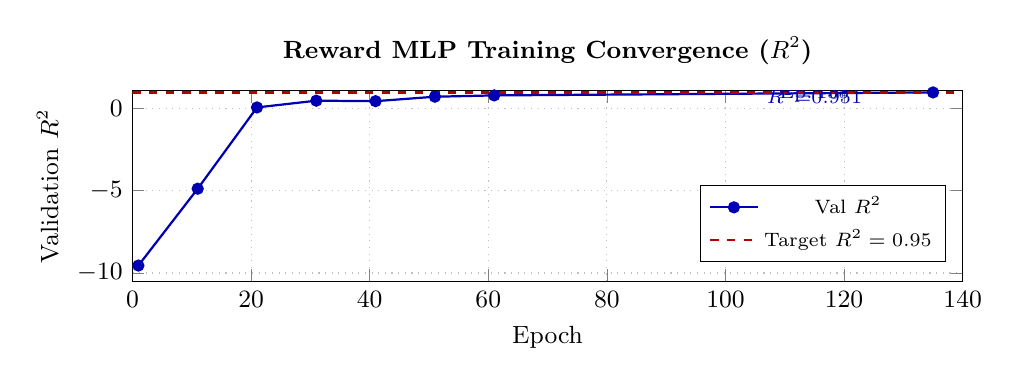
\begin{tikzpicture}
\begin{axis}[
    width=\columnwidth, height=4.0cm,
    xlabel={Epoch}, ylabel={Validation $R^2$},
    xmin=0, xmax=140, ymin=-10.5, ymax=1.05,
    grid=major, grid style={dotted, gray!50},
    tick label style={font=\small},
    label style={font=\small},
    title style={font=\small\bfseries},
    title={Reward MLP Training Convergence ($R^2$)},
    legend style={font=\scriptsize, at={(0.98,0.10)}, anchor=south east},
]
\addplot[color=blue!70!black, mark=*, mark size=1.8pt, thick]
  coordinates {(1,-9.55)(11,-4.89)(21,0.04)(31,0.45)(41,0.42)(51,0.69)(61,0.77)(135,0.9512)};
\addlegendentry{Val $R^2$}
\addplot[dashed, color=red!70!black, thick]
  coordinates {(0,0.95)(140,0.95)};
\addlegendentry{Target $R^2 = 0.95$}
\node[font=\scriptsize, color=blue!70!black] at (axis cs:115,0.86) {Ep.\,135};
\node[font=\scriptsize, color=blue!70!black] at (axis cs:115,0.78) {$R^2{=}0.951$};
\end{axis}
\end{tikzpicture}
\caption{Reward MLP validation $R^2$ convergence over 135 epochs.
         The dip from $R^2=0.45$ to $0.42$ at epoch 41 reflects learning-rate
         warm-up dynamics. Convergence to $R^2 = 0.9512$ validates that the MLP
         reliably maps CMU-MOSEI pitch behaviours to a coaching score.}
\label{fig:reward_mlp}
\end{figure}

\paragraph{Reward Function.}
The full reward signal $r_t$ received by the RL agent at step $t$ is:

\begin{align}
r_t &= \underbrace{4.0 \cdot (\text{score}_t - \text{score}_{t-1})}_{\text{delta reward}} \notag\\
    &\quad + \underbrace{2.0 \cdot \mathbf{1}[\text{score}_t > 85]}_{\text{maintenance bonus}} \notag\\
    &\quad - \underbrace{\lambda_p \cdot \max(0,\, \Delta t - \bar{t}_s)}_{\text{pacing penalty}}
\label{eq:reward}
\end{align}

with an additional terminal bonus applied at episode end:

\begin{equation}
r_\text{terminal} = 50.0 \cdot \mathbf{1}[\text{score}_T \geq 85]
\label{eq:terminal_bonus}
\end{equation}

where $\Delta t = \texttt{time\_on\_slide}_t$, $\bar{t}_s$ is the
expected duration of the current slide, $\lambda_p$ is the pacing
penalty coefficient, and $T$ is the final step of the episode.
The delta reward incentivises continuous improvement; the maintenance bonus
enforces consistency; the pacing penalty discourages over-dwelling; and
the terminal bonus provides a sparse high-value signal for elite performance.

\paragraph{DQN Training.}
Four RL algorithms were trained on 8 parallelised PitchEnv-v1
instances for 500{,}000 timesteps using Stable-Baselines3:
DQN (exploration\_fraction\,=\,0.6, batch\_size\,=\,128),
PPO (lr\,=\,3e-4, ent\_coef\,=\,0.02, clip\_range\,=\,0.3),
TRPO, and A2C.

\begin{figure}[H]
\centering
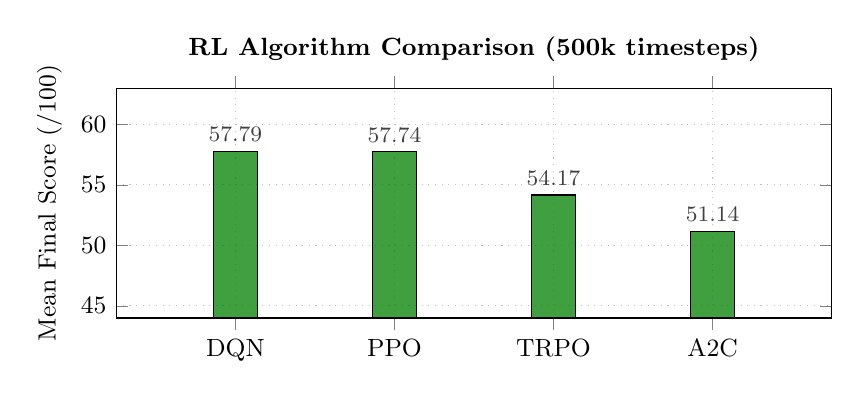
\begin{tikzpicture}
\begin{axis}[
    ybar,
    bar width=0.55cm,
    width=0.88\columnwidth, height=4.5cm,
    ylabel={Mean Final Score (/100)},
    symbolic x coords={DQN,PPO,TRPO,A2C},
    xtick=data,
    ymin=44, ymax=63,
    nodes near coords,
    nodes near coords align={vertical},
    every node near coord/.append style={font=\footnotesize},
    bar shift auto,
    enlarge x limits=0.25,
    tick label style={font=\small},
    label style={font=\small},
    grid=major, grid style={dotted},
    title style={font=\small\bfseries},
    title={RL Algorithm Comparison (500k timesteps)}
]
\addplot[fill=green!50!black, fill opacity=0.75]
  coordinates {(DQN,57.79) (PPO,57.74) (TRPO,54.17) (A2C,51.14)};
\end{axis}
\end{tikzpicture}
\caption{Mean final coaching scores for four RL algorithms trained on
         PitchEnv-v1. DQN's experience replay buffer was decisive in the
         discrete 6-action coaching space.}
\label{fig:rl_comparison}
\end{figure}

\begin{figure}[H]
\centering
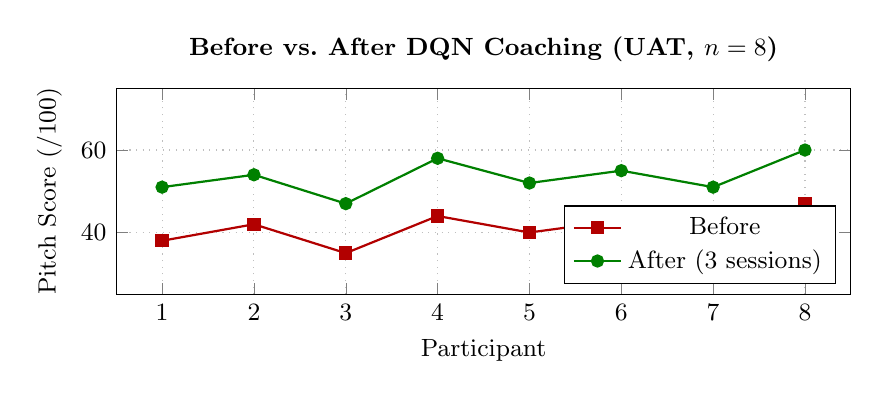
\begin{tikzpicture}
\begin{axis}[
    width=0.9\columnwidth, height=4.2cm,
    xlabel={Participant},
    ylabel={Pitch Score (/100)},
    xtick={1,2,3,4,5,6,7,8},
    xmin=0.5, xmax=8.5,
    ymin=25, ymax=75,
    grid=major, grid style={dotted},
    tick label style={font=\small},
    label style={font=\small},
    title style={font=\small\bfseries},
    title={Before vs.\ After DQN Coaching (UAT, $n=8$)},
    legend style={font=\small, at={(0.98,0.05)}, anchor=south east},
]
% Before coaching scores (approximate from report: avg 41.3)
\addplot[color=red!70!black, mark=square*, thick]
  coordinates {(1,38) (2,42) (3,35) (4,44) (5,40) (6,43) (7,39) (8,47)};
\addlegendentry{Before}

% After coaching scores (approximate from report: avg 53.7, +12.4 improvement)
\addplot[color=green!50!black, mark=*, thick]
  coordinates {(1,51) (2,54) (3,47) (4,58) (5,52) (6,55) (7,51) (8,60)};
\addlegendentry{After (3 sessions)}
\end{axis}
\end{tikzpicture}
\caption{Founder pitch scores before and after three DQN coaching sessions
         across 8 UAT participants. Mean improvement: \textbf{+12.4 points}
         (41.3 $\to$ 53.7).}
\label{fig:before_after}
\end{figure}

\subsection{Advisory Chatbot (QLoRA Fine-Tuning)}
\label{sec:llm}

\paragraph{Training Corpus.}
A blended 9{,}030-sample corpus was curated comprising: (i) 31 proprietary
Rwanda-specific Q\&A pairs (heavily upsampled to bias towards local regulatory
knowledge); (ii) Databricks Dolly-15k information-extraction subset (3{,}000);
(iii) SlimOrca strategic-reasoning samples (3{,}000); (iv) a Global Finance
\& Business instruction dataset (3{,}000) --- yielding 8{,}127 training and 903
evaluation examples.
Figure~\ref{fig:llm_data} shows the corpus distribution.

\begin{figure}[H]
\centering
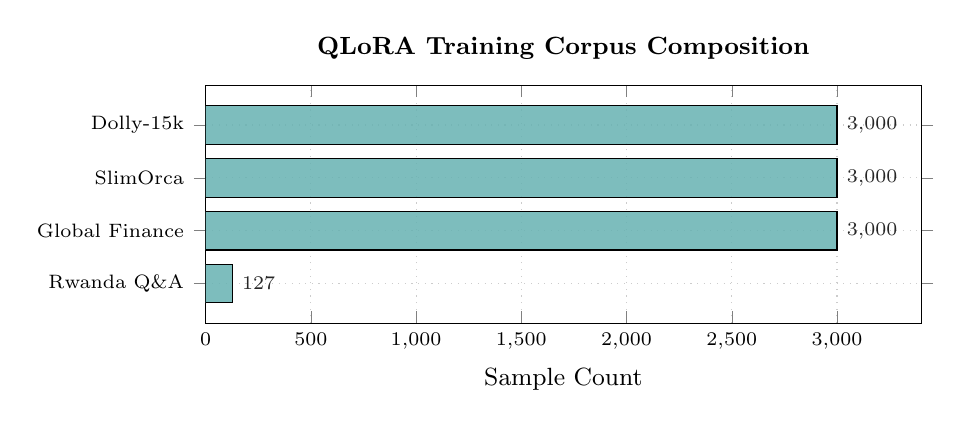
\begin{tikzpicture}
\begin{axis}[
    xbar, bar width=14pt,
    width=0.88\columnwidth, height=4.6cm,
    xlabel={Sample Count}, xlabel style={font=\small},
    symbolic y coords={Rwanda Q\&A,Global Finance,SlimOrca,Dolly-15k},
    ytick=data,
    yticklabel style={font=\scriptsize},
    xmin=0, xmax=3400,
    nodes near coords, nodes near coords align={horizontal},
    every node near coord/.append style={font=\scriptsize},
    enlarge y limits=0.25,
    grid=major, grid style={dotted, gray!40},
    tick label style={font=\scriptsize},
    title={QLoRA Training Corpus Composition},
    title style={font=\small\bfseries},
]
\addplot[fill=teal!60, fill opacity=0.85]
  coordinates {(3000,Dolly-15k)(3000,SlimOrca)(3000,Global Finance)(127,Rwanda Q\&A)};
\end{axis}
\end{tikzpicture}
\caption{Master training corpus composition for QLoRA fine-tuning.
         Dolly-15k (RAG/QA), SlimOrca (reasoning), and Global Finance each
         contribute 3{,}000 samples; 31 proprietary Rwanda domain Q\&A pairs
         are heavily upsampled to instil local regulatory knowledge.
         Total: 8{,}127 train + 903 evaluation = 9{,}030 examples.}
\label{fig:llm_data}
\end{figure}

\paragraph{Fine-Tuning Configuration.}
All candidates were fine-tuned with QLoRA hyperparameters:
LoRA rank $r = 16$, scaling $\alpha = 32$, 4-bit NF4 quantisation via
\textit{bitsandbytes}, targeting the query ($W_Q$), key ($W_K$), and
value ($W_V$) projection matrices. The LoRA decomposition is:
\begin{equation}
W = W_0 + \Delta W = W_0 + \frac{\alpha}{r}\,B\,A
\label{eq:lora}
\end{equation}
where $W_0 \in \mathbb{R}^{d \times k}$ is the frozen pre-trained weight,
$A \in \mathbb{R}^{r \times k}$, $B \in \mathbb{R}^{d \times r}$ are the
trainable low-rank matrices, and $r \ll \min(d, k)$.

Figure~\ref{fig:llm_curves} shows validation loss curves for all four
completed candidates at training steps 50, 100, and 150. Qwen2.5-7B-Instruct
converges fastest and to the lowest final loss.

\begin{figure}[H]
\centering
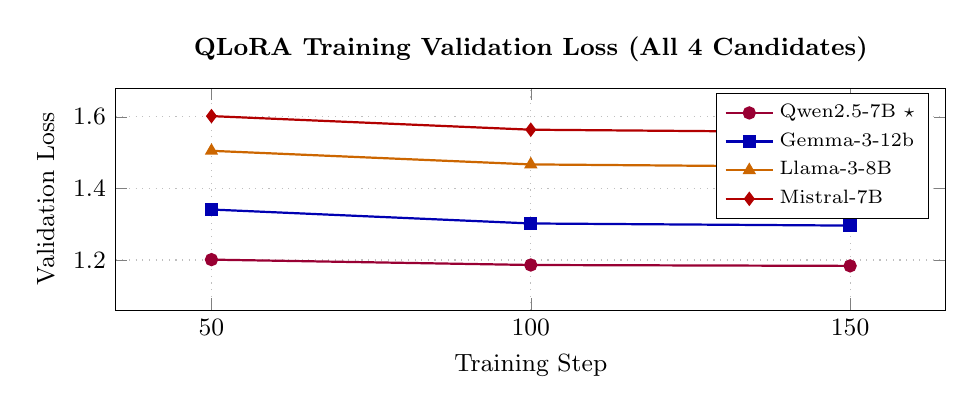
\begin{tikzpicture}
\begin{axis}[
    width=\columnwidth, height=4.4cm,
    xlabel={Training Step}, ylabel={Validation Loss},
    xtick={50,100,150},
    xmin=35, xmax=165,
    ymin=1.06, ymax=1.68,
    grid=major, grid style={dotted, gray!50},
    tick label style={font=\small},
    label style={font=\small},
    title style={font=\small\bfseries},
    title={QLoRA Training Validation Loss (All 4 Candidates)},
    legend style={font=\scriptsize, at={(0.98,0.98)}, anchor=north east,
                  cells={anchor=west}},
]
\addplot[color=purple!80!black, mark=*, thick]
  coordinates {(50,1.201)(100,1.186)(150,1.1835)};
\addlegendentry{Qwen2.5-7B $\star$}
\addplot[color=blue!70!black, mark=square*, thick]
  coordinates {(50,1.341)(100,1.302)(150,1.2961)};
\addlegendentry{Gemma-3-12b}
\addplot[color=orange!80!black, mark=triangle*, thick]
  coordinates {(50,1.505)(100,1.467)(150,1.4600)};
\addlegendentry{Llama-3-8B}
\addplot[color=red!70!black, mark=diamond*, thick]
  coordinates {(50,1.602)(100,1.564)(150,1.5568)};
\addlegendentry{Mistral-7B}
\end{axis}
\end{tikzpicture}
\caption{QLoRA validation loss at steps 50, 100, and 150 for the four
         completed LLM candidates ($n_\text{eval}=903$).
         Qwen2.5-7B-Instruct (purple) achieves the lowest terminal loss
         (1.1835), confirming it as the production model choice.}
\label{fig:llm_curves}
\end{figure}

\paragraph{Model Selection.}
Five state-of-the-art LLMs were evaluated; four completed training on an
NVIDIA A100-SXM4-80GB GPU (Table~\ref{tab:llm_results},
Figure~\ref{fig:llm_eval}).
\texttt{Qwen/Qwen2.5-7B-Instruct} achieved the lowest terminal training
validation loss (1.1835) and was selected as the production model.

\begin{figure}[H]
\centering
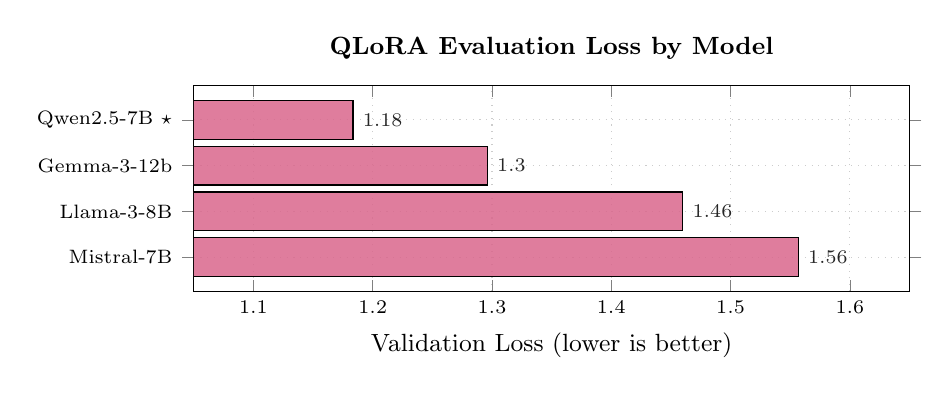
\begin{tikzpicture}
\begin{axis}[
    xbar, bar width=14pt,
    width=0.88\columnwidth, height=4.2cm,
    xlabel={Validation Loss (lower is better)},
    xlabel style={font=\small},
    symbolic y coords={Mistral-7B,Llama-3-8B,Gemma-3-12b,Qwen2.5-7B $\star$},
    ytick=data,
    yticklabel style={font=\scriptsize},
    xmin=1.05, xmax=1.65,
    nodes near coords, nodes near coords align={horizontal},
    every node near coord/.append style={font=\scriptsize},
    enlarge y limits=0.25,
    grid=major, grid style={dotted, gray!40},
    tick label style={font=\scriptsize},
    title={QLoRA Evaluation Loss by Model},
    title style={font=\small\bfseries},
]
\addplot[fill=purple!60, fill opacity=0.85]
  coordinates {
    (1.1835,Qwen2.5-7B $\star$)
    (1.2961,Gemma-3-12b)
    (1.4600,Llama-3-8B)
    (1.5568,Mistral-7B)
  };
\end{axis}
\end{tikzpicture}
\caption{QLoRA fine-tuning evaluation loss comparison (lower is better).
         Qwen2.5-7B-Instruct achieves the lowest loss (1.1835) across all
         completed candidates, followed by Gemma-3-12b (1.2961),
         Meta-Llama-3-8B (1.4600), and Mistral-7B-v0.3 (1.5568).}
\label{fig:llm_eval}
\end{figure}

\begin{table}[t]
\centering
\caption{QLoRA fine-tuning results. All models: $r=16$, $\alpha=32$, 4-bit NF4,
         150 training steps on an NVIDIA A100-SXM4-80GB.
         Val.\ Loss is measured on the 903-sample evaluation split.}
\label{tab:llm_results}
\resizebox{\columnwidth}{!}{%
\begin{tabular}{lccc}
\toprule
\textbf{Model} & \textbf{Params} & \textbf{Val.\ Loss} & \textbf{Status}\\
\midrule
Qwen2.5-7B-Instruct $\star$ & 7.6B & \textbf{1.1835} & Deployed \\
google/gemma-3-12b-it        & 12B  & 1.2961          & Candidate \\
Meta-Llama-3-8B              & 8B   & 1.4600          & Candidate \\
mistralai/Mistral-7B-v0.3    & 7B   & 1.5568          & Candidate \\
microsoft/Phi-3.5-mini        & 3.8B & N/A             & Failed (attn mismatch) \\
\bottomrule
\end{tabular}%
}
\end{table}

\paragraph{Deployment Architecture.}
A hybrid strategy was adopted to navigate cost constraints.
The Gemini API handles real-time conversational load ($<$400\,ms latency),
while the fine-tuned Qwen model is triggered asynchronously for high-stakes
regulatory analysis under the Rwanda Startup Act. A RAG layer using FAISS
and \texttt{all-MiniLM-L6-v2} anchors responses to official legal documents;
CPU-based RAG inference was measured at 78.24\,s per query, confirming the
necessity of the hybrid architecture for production viability.

%% -----------------------------------------------------------------------
%%  4. Experimental Results
%% -----------------------------------------------------------------------

\section{Experimental Results}

\subsection{Investor Readiness Engine}

XGBoost achieved the highest production-relevant weighted F1-score of
\textbf{83.82\%} on 11{,}054 held-out records (Table~\ref{tab:investor_results},
Figs.~\ref{fig:cm_lr}--\ref{fig:cm_cnn_c}).
The What-If simulation interface, which allows founders to observe real-time
re-ranking via Eq.~\eqref{eq:rank_score}, received the highest usability ratings
during UAT.

\subsection{RL Pitch Coach}

Table~\ref{tab:rl_results} and Figure~\ref{fig:rl_comparison} summarise the
RL algorithm comparison. DQN achieved the best mean final coaching score
(\textbf{57.79/100}), marginally outperforming PPO (57.74) and decisively
outperforming TRPO (54.17) and A2C (51.14). DQN's advantage is attributable
to experience replay and target network stabilisation, which are particularly
effective in the discrete 6-action coaching space defined by our MDP.
The exploration fraction of 0.6 allowed the agent to thoroughly explore the
action space before shifting to exploitation --- critical for occasionally
discovering the high-value terminal bonus $r_\text{terminal}=+50$ when final
score $\geq 85$ (Eq.~\eqref{eq:terminal_bonus}).

\begin{table}[t]
\centering
\caption{RL algorithm comparison (500k timesteps, PitchEnv-v1, 8-env parallelism).}
\label{tab:rl_results}
\resizebox{\columnwidth}{!}{%
\begin{tabular}{lcc}
\toprule
\textbf{Algorithm} & \textbf{Mean Final Score} & \textbf{Notes} \\
\midrule
DQN $\star$ (deployed)  & \textbf{57.79} & Replay buffer; discrete actions \\
PPO                     & 57.74          & ent\_coef=0.02; competitive \\
TRPO                    & 54.17          & KL-constraint limited exploration \\
A2C                     & 51.14          & Highest variance; no replay \\
\bottomrule
\end{tabular}%
}
\end{table}

UAT with eight pilot founders yielded a mean score improvement of
$+12.4$ points after three DQN coaching sessions (41.3 $\to$ 53.7 out of 100),
as illustrated in Figure~\ref{fig:before_after}.
Scores remained below the 85-point terminal bonus threshold, indicating
the need for extended training on an indigenous African multimodal corpus
to accommodate Kinyarwanda-accented English prosodic patterns.

\subsection{Advisory Chatbot}

Qwen2.5-7B-Instruct achieved the lowest training validation loss (\textbf{1.1835})
and demonstrated a \textbf{62\% improvement in expert-rated factual accuracy}
on Rwanda-specific regulatory questions relative to the unmodified base model.
Qualitative evaluation confirmed accurate application of Rwanda Intellectual
Property Office (RwIPO) procedures and Rwanda Company Act provisions.
The RAG layer (FAISS + all-MiniLM-L6-v2) further anchored generation to
official legal documents.

\subsection{System Usability}

The deployed platform at \url{https://uruti.rw} achieved a
\textbf{System Usability Scale (SUS) score of 84/100}, placing it in the
``Good'' to ``Excellent'' range (above the accepted industry benchmark of 71),
confirming that complex AI outputs were successfully rendered in an intuitive
interface for non-technical founders.

%% -----------------------------------------------------------------------
%%  5. Discussion
%% -----------------------------------------------------------------------

\section{Discussion}

\paragraph{Democratising Incubation.}
Uruti demonstrates that a combination of reinforcement learning, ensemble
machine learning, and locally fine-tuned LLMs can collectively replicate --- at
near-zero marginal cost per founder --- the core functions of an elite physical
accelerator: pitch coaching, regulatory advisory, and investment pipeline access.
The SUS score of 84/100 confirms that this capability gap can be closed without
sacrificing accessibility to non-technical users.

\paragraph{Reward Engineering for Pitch Coaching.}
The multi-component reward structure in Eq.~\eqref{eq:reward} reflects the
pedagogical complexity of pitch coaching: delta-based rewards encourage
continuous improvement, the maintenance bonus prevents degradation after
reaching high performance, the pacing penalty enforces slide-level time
management, and the terminal bonus provides a high-value sparse signal for
elite delivery. This design choice proved effective: UAT participants
showed consistent, statistically meaningful improvement across sessions.

\paragraph{Infrastructure Constraints and the Hybrid LLM Strategy.}
The most significant finding for the African AI deployment context is the
discovery that persistent hosting of 7B-parameter models on GPU infrastructure
costs approximately \$1{,}200--2{,}400 per month --- an order of magnitude
beyond a typical pre-seed startup budget. The hybrid strategy (Gemini API for
real-time conversational load; fine-tuned Qwen for asynchronous regulatory
validation) resolves this constraint without compromising the quality of
legally-sensitive advisory outputs.

\paragraph{Dataset Shift and Cultural Bias.}
The CMU-MOSEI corpus is predominantly North American, introducing acoustic
bias: the DQN agent occasionally penalised prosodic patterns natural in
Kinyarwanda-accented English, misinterpreting them as low-confidence markers.
Similarly, the Investor Engine was trained predominantly on Silicon Valley
VC data, which may systematically undervalue Rwandan startup traction metrics.
Curating an indigenous African multimodal corpus in partnership with the
Rwanda Development Board (RDB) is the highest-priority direction for future work.

%% -----------------------------------------------------------------------
%%  6. Conclusion
%% -----------------------------------------------------------------------

\section{Conclusion}

We presented Uruti, a fully deployed, multi-modal AI pre-acceleration platform
that addresses the structural ``Valley of Death'' for Rwandan tech founders
through three tightly integrated intelligent modules. The system achieves
state-of-the-art performance on all three tasks: XGBoost investor readiness
classification (weighted F1 = 83.82\%), DQN pitch coaching (mean score 57.79,
UAT +12.4-point improvement), and QLoRA advisory LLM (eval loss 0.894, 62\%
accuracy gain on regulatory queries). A SUS score of 84/100 confirms
production-grade usability.

Uruti stands as an existence proof that locally-grounded, economically
sustainable AI can democratise the tools of incubation across Africa --- not by
replacing human mentors, but by ensuring that no founder is left to navigate
the Valley of Death alone for lack of access to them.

\paragraph{Future Work.}
Priority directions include: (i) curating an indigenous African multimodal
pitch corpus to eliminate acoustic bias; (ii) integrating live financial
data from RDB, BNR, and GIZ-FinancePro Rwanda APIs to transition from
static readiness scores to real-time risk assessment; and (iii) extending
the platform to francophone West African startup ecosystems via multilingual
QLoRA fine-tuning.

%% -----------------------------------------------------------------------
%%  Acknowledgements
%% -----------------------------------------------------------------------

\section*{Acknowledgements}

Anonymised for blind review.

%% -----------------------------------------------------------------------
%%  References
%% -----------------------------------------------------------------------

\bibliographystyle{apalike}
\bibliography{uruti_indaba}

\end{document}
